\documentclass[11pt,a4paper]{article}

% ============================================
% PACKAGES
% ============================================

% Encoding and fonts
\usepackage[utf8]{inputenc}
\usepackage[T1]{fontenc}
\usepackage{mathptmx}  % Times New Roman

% Remove section numbering
\setcounter{secnumdepth}{0}

% Page layout
\usepackage[margin=2.5cm]{geometry}
\usepackage{setspace}
\onehalfspacing
\usepackage{ragged2e}
\justifying  % Ensure fully justified text

% Disable hyphenation - move whole words to next line
\hyphenpenalty=10000
\exhyphenpenalty=10000
\tolerance=1000
\emergencystretch=\maxdimen

% No paragraph indentation
\setlength{\parindent}{0pt}
\setlength{\parskip}{1em}  % Add space between paragraphs instead

% Graphics and figures
\usepackage{graphicx}
\usepackage{float}
\usepackage{subcaption}
\graphicspath{{figures/}}

% Caption styling - 9pt font, labels underneath
\usepackage{caption}
\captionsetup{font=small,skip=10pt}
\captionsetup[table]{position=below}
\captionsetup[figure]{position=below}

% Tables
\usepackage{booktabs}
\usepackage{longtable}
\usepackage{tabularx}
\usepackage{multirow}

% Left-align text in table X columns
\newcolumntype{L}{>{\raggedright\arraybackslash}X}

% Math
\usepackage{amsmath}
\usepackage{amssymb}

% Code listings
\usepackage{listings}
\usepackage{xcolor}
\usepackage{colortbl}

\definecolor{codegreen}{rgb}{0,0.6,0}
\definecolor{headergray}{rgb}{0.9,0.9,0.9}
\definecolor{codegray}{rgb}{0.5,0.5,0.5}
\definecolor{codepurple}{rgb}{0.58,0,0.82}
\definecolor{backcolour}{rgb}{0.95,0.95,0.92}

\lstdefinestyle{mystyle}{
    backgroundcolor=\color{backcolour},
    commentstyle=\color{codegreen},
    keywordstyle=\color{magenta},
    numberstyle=\tiny\color{codegray},
    stringstyle=\color{codepurple},
    basicstyle=\ttfamily\footnotesize,
    breakatwhitespace=false,
    breaklines=true,
    captionpos=b,
    keepspaces=true,
    numbers=left,
    numbersep=5pt,
    showspaces=false,
    showstringspaces=false,
    showtabs=false,
    tabsize=2
}
\lstset{style=mystyle}

% Hyperlinks
\usepackage[hidelinks]{hyperref}
\usepackage{url}
\urlstyle{same}

% Bibliography
\usepackage[
    backend=biber,
    style=authoryear,
    sorting=nyt,
    maxcitenames=2
]{biblatex}
\addbibresource{references.bib}

% Glossaries and acronyms
\usepackage[acronym,toc]{glossaries}
\makeglossaries

% Headers and footers
\usepackage{fancyhdr}
\pagestyle{fancy}
\fancyhf{}
\fancyhead[L]{\nouppercase{\leftmark}}
\fancyhead[R]{\thepage}
\renewcommand{\headrulewidth}{0.4pt}

% Appendices
\usepackage[toc,page]{appendix}

% Section formatting - match appendix header style with page breaks
\usepackage{titlesec}
\titleformat{\section}{\normalfont\fontsize{20}{24}\selectfont\bfseries}{\thesection}{1em}{}
\titleformat{\subsection}{\normalfont\large\bfseries}{\thesubsection}{1em}{}
\titleformat{\subsubsection}{\normalfont\normalsize\bfseries}{\thesubsubsection}{1em}{}
\newcommand{\sectionbreak}{\clearpage}

% Gantt charts
\usepackage{pgfgantt}

% ============================================
% ACRONYMS
% ============================================

\newacronym{pb}{PB}{Pitch Book}
\newacronym{ib}{IB}{Investment Banking}
\newacronym{rag}{RAG}{Retrieval-Augmented Generation}
\newacronym{llm}{LLM}{Large Language Model}
\newacronym{vlm}{VLM}{Vision Language Model}
\newacronym{pm}{PM}{Precedent Material}
\newacronym{api}{API}{Application Programming Interface}
\newacronym{sdlc}{SDLC}{Software Development Lifecycle}
\newacronym{poc}{POC}{Proof of Concept}
\newacronym{hitl}{HITL}{Human-in-the-Loop}

% ============================================
% DOCUMENT INFO
% ============================================

\title{Compliance Aware, Agentic Pitch Book Generation For Bankers}
\author{Andrei Rizea}
\date{\today}

% ============================================
% DOCUMENT
% ============================================

\begin{document}

% --------------------------------------------
% FRONT MATTER
% --------------------------------------------

% Title Page
\begin{titlepage}
    \centering
    \vspace*{2cm}

    {\Huge\bfseries Compliance Aware, Agentic Pitch Book Generation For Bankers\par}

    \vspace{1cm}

    {\Large A template-aware PowerPoint generation system with agentic data retrieval for investment banking.\par}

    \vfill

    {\Large A Queen Mary Final Year Dissertation\par}

    \vspace{1cm}

    {\large\bfseries Andrei Rizea\par}
    {\large Student ID: 220300153\par}

    \vspace{1cm}

    {\large Supervised by: Manesha Peiris\par}

    \vspace{1cm}

    {\large Programme of Study:\par}
    {\large Digital \& Technology Solutions (Software Engineering)\par}

    \vspace{1cm}

    {\large Module: IOT635W\par}

    \vfill

    \vspace{1cm}

    {\large Queen Mary University of London\par}
    {\large \today\par}

\end{titlepage}

% --------------------------------------------
% ABSTRACT
% --------------------------------------------
\newpage
\section*{Abstract}
\addcontentsline{toc}{section}{Abstract}

% TODO: Write abstract

% --------------------------------------------
% TABLE OF CONTENTS
% --------------------------------------------
\newpage
{\setlength{\parskip}{0pt}
\tableofcontents
}

\newpage
{\setlength{\parskip}{0pt}
\singlespacing
\listoffigures
}

\newpage
{\setlength{\parskip}{0pt}
\singlespacing
\listoftables
}

{\setlength{\parskip}{0pt}
\printglossary[type=\acronymtype,title=List of Acronyms]
}

% --------------------------------------------
% MAIN MATTER
% --------------------------------------------

\section{Introduction, Scope and Context}
\label{sec:introduction}

McKinsey found knowledge workers spend a fifth of their time searching for information \parencite{mckinsey2012social}. Investment banking (IB) is worse. By some estimates, document preparation eats up half to three-quarters of a junior banker's week, and pitch books (PBs) account for a big chunk of that \parencite{cfi2025analyst, wso2024hours}. When Goldman Sachs surveyed its first-year analysts in 2021, the average was 98 hours a week, and preparing documents was a major driver of the burnout they reported \parencite{bbc2021goldmanjuniors}. Yet most PBs look nearly identical to one another. Change the company name and update the numbers, and you could reuse last month's deck. This repetitiveness makes them well suited to automation.

IB firms advise companies on mergers, acquisitions, capital raising, and other financial transactions. The work is high-stakes. A single deal might be worth billions of dollars, and the documents that support these deals need to be accurate, professional, and persuasive. PBs are the primary vehicle for communicating analysis to clients and internal stakeholders. They summarise a company's financial position, compare it to peers, and make the case for why a particular transaction makes sense. Getting these documents right matters, but getting them done quickly matters too.

The industry has tried various approaches to this problem. Some firms have built internal document libraries where analysts can search for past work. Others have hired dedicated presentation specialists to handle formatting. A few have experimented with automation tools. None of these solutions have fully addressed the underlying issue: too much skilled human time goes toward work that does not require skill.

\subsection{Where Analyst Time Goes}
\label{sec:analyst-time}

IB sells expertise rather than physical goods, so you would expect analyst time to go toward analysis and client relationships. Often it does not.

A typical PB contains an executive summary, company overview, market analysis, valuation work, transaction comparables, and next steps. These sections appear in nearly every deck, along with the same content types: company descriptions, financial tables, market charts, and deal diagrams. The data inside changes, but the shell around it rarely does.

Analyst tasks fall into two buckets. The first holds work that genuinely needs a trained banker: financial modelling, valuation analysis, due diligence, and client advisory. The second holds everything else: hunting down data, reformatting slides, and fixing fonts. Too many hours go into the second bucket.

The process typically works like this. A managing director wins a new engagement and assigns it to an analyst team. The analysts start by digging through the firm's document archives, looking for similar deals they can use as templates. They pull financial data from Bloomberg terminals, public filings, and company reports. They copy and paste this information into PowerPoint, reformatting it to match the firm's visual standards. Then they send a draft up the chain for review. Senior bankers mark it up with corrections, and the analysts revise and resubmit. This cycle might repeat several times before the document is ready for the client.

Each step in this process has friction. The document archive search is often slow and incomplete. Data entry is error-prone. Formatting is tedious. Review cycles eat up time on both ends. The result is that a significant portion of analyst hours goes toward activities that could, in theory, be automated.

Banks pay junior analysts well, so time spent on low-skill tasks represents a poor return on that investment. Shifting even some of that document preparation time back toward analytical work would improve the economics. This is not about replacing analysts. It is about freeing them to do analyst work.

Research supports this view. Radhakrishna et al. found that well-designed knowledge management systems boosted productivity by 20 to 25 percent \parencite{radhakrishna2024km}. Document production was identified as a prime candidate for automation, provided humans retained control over judgement calls.

\subsection{Problem Analysis}
\label{sec:problem-analysis}

Markus defined knowledge reuse in 2001, and her framework fits PB production well \parencite{markus2001knowledge}. She identified several reuse patterns: drawing on past work, borrowing from colleagues, finding subject matter experts, and mining old documents. PB creation involves all of these, often in the same afternoon.

Three things get in the way.

First, too much time goes to low-value work. Analysts spend hours searching through old decks, extracting useful content, and reformatting slides to fit the current template. None of that requires analytical thinking, yet it crowds out the work that does.

Second, institutional knowledge tends to disappear. Researchers distinguish between tacit knowledge, which stays in people's heads, and explicit knowledge, which gets written down \parencite{dalkir2011km}. PBs themselves are explicit since they capture analysis in a shareable format. But the knowledge of how to make a good PB remains tacit: which templates work for which situations, how to structure the narrative, what separates a persuasive pitch from a forgettable one. New analysts pick this up by watching senior colleagues, not by reading a manual.

Third, onboarding takes longer than it should. Each bank has its own templates, preferred data sources, writing conventions, and quality expectations. Junior analysts absorb these through trial and error, which is slow for them and a drain on the senior bankers who review their work. A new analyst might spend weeks learning which template to use for which situation, how to format financial tables correctly, and what level of detail is expected in different sections. This knowledge exists somewhere in the organisation, but finding it and absorbing it takes time.

These three problems reinforce each other. When knowledge is scattered, people waste time searching for it. When standards live in people's heads rather than in documents, output quality varies and review cycles drag on. When training happens informally, experienced staff lose hours to coaching that could have gone toward billable work. A system that tackled even one of these issues would help, but one that addressed all three could meaningfully change how PB production works.

\subsection{Gap Analysis}
\label{sec:gap-analysis}

Automated presentation tools have existed for years. Early versions converted text to slides using layout algorithms, but although the content was organised, the slides looked bad and nobody wanted to use them \parencite{zheng2025pptagent}. Template-based systems came next, where you define the structure upfront and the system fills in the blanks. That fixed the visual problems but made everything rigid.

PPTAgent takes a different approach \parencite{zheng2025pptagent}. It analyses reference presentations, extracts their structural patterns, and applies those patterns to new content. Because it learns from real examples rather than following hardcoded rules, it beat older text-to-slide systems on both content quality and design quality in testing.

The catch is that PPTAgent targets general-purpose presentations, and IB PBs are anything but general. They have financial tables with specific column layouts, transaction comparables formatted in particular ways, and market positioning charts that follow visual conventions the industry recognises. Generic tools miss these conventions entirely, and in IB, getting the template wrong kills credibility. You could have the best analysis in the world, but if the deck looks off, nobody will take it seriously.

Commercial tools share this flaw. Beautiful.ai, Tome, and Gamma can all generate slides from a prompt, but the output is generic and every slide needs rework to match firm standards. None of them connect to financial data sources either, so analysts still have to gather numbers and enter them by hand. These tools work well for general business presentations, but they were not built for the specific demands of financial services.

The fundamental challenge is that IB PBs require both domain knowledge and visual precision. The content needs to reflect financial expertise. The formatting needs to match exacting corporate standards. Generic AI tools typically handle one or the other, but not both. A system that could combine financial data retrieval, domain-appropriate content generation, and template-aware slide assembly would address a genuine unmet need.

Here is the gap. Current systems either produce generic output that needs heavy cleanup, or they require large training datasets to learn industry-specific patterns. Most banks lack those datasets. What nobody seems to have built yet is a system that can take a single reference template, extract its styling and layout rules programmatically, and generate new slides that follow those rules exactly. That kind of template-aware approach would let firms preserve their visual identity while offloading the tedious formatting work.

Agentic AI architectures look promising for this \parencite{ibm2024agentic}. Instead of one model doing everything in a single pass, the system breaks tasks into steps and uses the right tool for each one. Wang et al. surveyed LLM-based agents and found that progress has been rapid \parencite{wang2023llmagents}. McKinsey estimates generative AI could deliver \$340 billion annually in banking \parencite{mckinsey2024genaibanking}. Document-heavy workflows sit right in the sweet spot.

My project addresses this gap. The pipeline extracts layouts, colour palettes, and placeholder positions from a template using python-pptx, uses an LLM to plan content, then assembles slides matching the original style. I am using existing agentic frameworks rather than custom orchestration. RAG against past PBs is a stretch goal.

The approach differs from prior work in two important ways. First, it prioritises template fidelity over content generation. The system starts with the visual constraints and works backward to content, rather than generating content and hoping the formatting works out. Second, it uses an agentic architecture where specialised components handle distinct parts of the task. One component analyses templates, another retrieves data, another plans content, and another assembles slides. This separation makes the system easier to test and modify.

\subsection{Aims and Objectives}
\label{sec:aims-objectives}

The aim is to design, build, and test a proof-of-concept (POC) demonstrating how AI-powered document generation can tackle the knowledge reuse problems described above. The system must respect institutional templates throughout. If it generates slides that do not match the house style, the whole thing fails.

On the business side, I want a workflow where an analyst can provide minimal input and get back a solid first draft. That would cut the time spent on formatting grunt work while keeping humans in control of the actual analysis. The target users are junior analysts, the people who currently spend most of their hours on document preparation.

On the learning side, I want to understand how to connect LLM orchestration with programmatic document generation. That means getting into agentic architectures, learning how to extract patterns from templates, and working out how to combine multiple AI capabilities into something that functions end to end. I am also interested in human-in-the-loop (HITL) design, since in a regulated industry like finance, AI tools need to support professional judgement rather than try to replace it. The banking sector faces significant regulatory scrutiny, and any AI system deployed in this context must be transparent, auditable, and controllable by human operators.

Five objectives structure the work:

\begin{enumerate}
    \item Build a template analysis component that takes a reference PowerPoint file and extracts its layout structures, colour palettes, font specifications, and placeholder positions.
    \item Build an agentic data retrieval layer that automatically pulls company financials, market data, and regulatory filings from Yahoo Finance and SEC EDGAR.
    \item Build an LLM-powered content planning module that produces structured slide specifications adapted to different PB types while keeping the overall narrative coherent.
    \item Build a slide assembly component that takes the content plan and template patterns and produces a PowerPoint file meeting formatting standards.
    \item Evaluate the system by measuring generation speed, template matching, and content quality.
\end{enumerate}

\subsection{Scope and Success Criteria}
\label{sec:scope}

The POC takes user input (company, transaction type, dates, reference template, PB type) and produces a formatted PowerPoint. Target PB types are company overviews, market updates, and transaction summaries. Full valuation presentations are out of scope.

Design choices: established agentic frameworks rather than custom architecture, programmatic template extraction with python-pptx rather than vision models, public APIs only, and RAG as a stretch goal. Out of scope: real-time data feeds, production infrastructure, compliance validation. Deal positioning and valuation judgements stay with analysts. Practical limits: one academic term, standard hardware, student API budget.

Success criteria:

\begin{itemize}
    \item Generate complete PB draft within five minutes
    \item Match reference template formatting
    \item Accurate financial data from source APIs
    \item Content structure following IB conventions, verified against precedent examples
\end{itemize}

One principle runs through all of this: HITL design. The system produces drafts for human review, not finished products. The goal is a solid starting point rather than a blank slide. This approach acknowledges that AI systems are not yet capable of the nuanced judgement that financial analysis requires, but they can handle the mechanical work that currently absorbs too much human attention.

% --------------------------------------------
% SUBSEQUENT SECTIONS
% --------------------------------------------

\section{Methodology and Project Plan}
\label{sec:methodology}

This section covers how I will approach development, what the requirements are, which technologies I have chosen and why, the project schedule, and how I am thinking about risks and ethics. Reproducibility is a guiding principle throughout. I want anyone reading this work to be able to understand my choices, replicate my setup, and reproduce my results.

\subsection{Development Methodology}
\label{sec:dev-methodology}

Software development methodologies range from plan-driven approaches like Waterfall to adaptive approaches like Agile \parencite{sommerville2016software}. Choosing the right methodology depends on requirement stability, project complexity, stakeholder availability, and team size. Table~\ref{tab:methodology-comparison} compares methodologies against criteria relevant to this project.

\begin{table}[H]
\centering
\begin{tabularx}{\textwidth}{|l|L|L|L|}
\hline
\textbf{Criteria} & \textbf{Waterfall} & \textbf{Scrum} & \textbf{Iterative Prototyping} \\
\hline
Requirements stability & Requires fixed requirements upfront & Accommodates changing requirements & Works well when requirements change \\
\hline
Feedback loops & Late feedback after implementation & Sprint reviews every 2-4 weeks & Continuous feedback through prototypes \\
\hline
Risk management & Risks discovered late & Regular risk reassessment & Early risk identification through prototypes \\
\hline
Solo developer suitability & Moderate & Low (designed for teams) & High \\
\hline
Research integration & Poor & Moderate & Excellent \\
\hline
\end{tabularx}
\caption{Comparison of Development Methodologies}
\label{tab:methodology-comparison}
\end{table}

I will use a hybrid methodology combining iterative prototyping with structured research engineering practices. Pure Waterfall cannot accommodate the exploratory nature of this work. Full Scrum adds overhead without benefit for a solo developer. Iterative prototyping lets me adapt as I learn, while structured practices keep the work repeatable.

The choice of iterative prototyping reflects the nature of the problem. I am building a system that combines several technologies in ways that have not been done before. Some technical decisions will only make sense after I have tried them. For example, I cannot know in advance whether a particular prompt structure will produce good slide content until I have tested it with real data. The methodology needs to accommodate this kind of learning.

At the same time, this is academic work that others should be able to evaluate and build upon. That means I need to document my decisions, track my progress, and make my process transparent. The structured practices serve this purpose.

Each two-week iteration will produce a working prototype targeting defined requirements. At each cycle's end, I will conduct a retrospective review and document outcomes. Feedback from IB practitioners, where possible, will shape subsequent cycles. The iteration cycle follows a consistent pattern: plan what to build, build it, test it, document what I learned, and decide what to do next.

I will use Git with a simplified GitFlow model (main, develop, feature branches). Continuous integration via GitHub Actions will run tests and linting on every push, enforcing 80\% coverage for core modules. I will maintain a decision log using Architecture Decision Records (ADRs) to document technical choices and trade-offs. Each ADR captures the context, the decision, the alternatives considered, and the consequences. This creates an audit trail that explains not just what I built but why I built it that way.

\subsection{Requirements Analysis}
\label{sec:requirements}

Good requirements are needed to measure whether the project succeeded. This section separates business requirements (the value delivered) from functional requirements (what the system does) and non-functional requirements (how well it performs).

I gathered requirements from several sources. The problem analysis in the introduction identified core pain points from industry reports and academic literature. My own experience working in financial services informed the technical constraints. Published research on document generation and agentic AI systems shaped the functional approach. The requirements below synthesise these inputs into testable statements.

Requirements follow the MoSCoW prioritisation scheme. "Must have" requirements define the minimum viable product. "Should have" requirements add important functionality that time permitting will be included. "Could have" requirements represent stretch goals. "Won't have" requirements clarify scope boundaries.

\subsubsection{Business Requirements}

Business requirements describe the value the project should deliver. These connect technical work to real-world outcomes:

\begin{enumerate}
    \item \textbf{BR1: Productivity Enhancement}: Reduce time spent on initial PB drafting by generating solid first drafts from minimal input.
    \item \textbf{BR2: Knowledge Codification}: Capture institutional presentation standards through template analysis, reducing reliance on tacit knowledge.
    \item \textbf{BR3: Quality Consistency}: Follow corporate visual identity standards consistently, reducing revision cycles caused by formatting issues.
    \item \textbf{BR4: Data Accuracy}: Financial data in generated PBs should accurately reflect source information.
\end{enumerate}

\subsubsection{Functional Requirements}

Table~\ref{tab:functional-requirements} lists functional requirements by component using MoSCoW prioritisation (Must have, Should have, Could have, Won't have).

\begin{table}[H]
\centering
\begin{tabularx}{\textwidth}{|l|l|L|l|}
\hline
\textbf{ID} & \textbf{Component} & \textbf{Requirement} & \textbf{Priority} \\
\hline
FR1 & Template Analyser & Extract slide layouts from reference .pptx files & Must \\
\hline
FR2 & Template Analyser & Identify colour palettes and font specifications & Must \\
\hline
FR3 & Template Analyser & Map placeholder positions and content types & Must \\
\hline
FR4 & Data Retrieval & Fetch company financials from Yahoo Finance API & Must \\
\hline
FR5 & Data Retrieval & Retrieve SEC filings via EDGAR API & Should \\
\hline
FR6 & Data Retrieval & Perform web searches for company news & Should \\
\hline
FR7 & Content Planner & Generate slide-by-slide content specifications & Must \\
\hline
FR8 & Content Planner & Adapt content structure to PB type & Must \\
\hline
FR9 & Content Planner & Maintain narrative coherence across slides & Should \\
\hline
FR10 & Slide Builder & Assemble slides matching template layouts & Must \\
\hline
FR11 & Slide Builder & Populate placeholders with generated content & Must \\
\hline
FR12 & Slide Builder & Generate charts from financial data & Could \\
\hline
FR13 & Orchestration & Coordinate multi-step generation workflow & Must \\
\hline
FR14 & Orchestration & Handle API failures gracefully & Should \\
\hline
FR15 & RAG Search & Query precedent material repository & Could \\
\hline
\end{tabularx}
\caption{Functional Requirements Specification}
\label{tab:functional-requirements}
\end{table}

\subsubsection{Non-Functional Requirements}

Table~\ref{tab:nonfunctional-requirements} lists quality requirements with measurable acceptance criteria.

\begin{table}[H]
\centering
\begin{tabularx}{\textwidth}{|l|l|L|L|}
\hline
\textbf{ID} & \textbf{Category} & \textbf{Requirement} & \textbf{Acceptance Criterion} \\
\hline
NFR1 & Performance & System generates complete PB draft & Within 5 minutes of input submission \\
\hline
NFR2 & Performance & API response handling & Timeout after 30 seconds with graceful degradation \\
\hline
NFR3 & Reliability & System availability during demonstration & 95\% uptime during evaluation period \\
\hline
NFR4 & Usability & Input specification interface & Requires no technical expertise to operate \\
\hline
NFR5 & Maintainability & Codebase documentation & All public functions documented with docstrings \\
\hline
NFR6 & Security & API credential management & No credentials in source code; environment variables used \\
\hline
NFR7 & Security & Input validation & All user inputs sanitised before processing \\
\hline
NFR8 & Compatibility & Output format & Valid .pptx files openable in Microsoft PowerPoint \\
\hline
\end{tabularx}
\caption{Non-Functional Requirements Specification}
\label{tab:nonfunctional-requirements}
\end{table}

\subsection{Technology Stack}
\label{sec:technology-stack}

I chose technologies based on four factors:

\begin{itemize}
    \item \textbf{Task fit}: Does the tool solve the specific problem well?
    \item \textbf{Familiarity}: Do I already know how to use it?
    \item \textbf{Ecosystem maturity}: Is it well-documented with active community support?
    \item \textbf{Maintainability}: Will it be easy to debug and extend?
\end{itemize}

\subsubsection{Programming Language and Framework}

I chose Python as the main language because it dominates AI and ML development and has a large library ecosystem. I am also comfortable with Python from my work experience, which means I can focus on the problem rather than learning a new language. Table~\ref{tab:language-comparison} compares Python with alternatives.

\begin{table}[H]
\centering
\begin{tabularx}{\textwidth}{|l|L|L|L|}
\hline
\textbf{Criteria} & \textbf{Python} & \textbf{JavaScript/Node.js} & \textbf{Java} \\
\hline
Benefits & Best AI/ML libraries, mature PowerPoint library (python-pptx), rapid development & Native async, same language frontend and backend & Strong typing, enterprise support \\
\hline
Risks & Slower execution than compiled languages, GIL limits true parallelism & AI/ML ecosystem less mature, limited PowerPoint options & Verbose code, slower development \\
\hline
AI/ML support & Excellent (PyTorch, LangChain, OpenAI SDK) & Growing but limited & Moderate (DJL, Langchain4j) \\
\hline
PowerPoint manipulation & python-pptx (mature, well-documented) & Limited options & Apache POI (verbose API) \\
\hline
\end{tabularx}
\caption{Programming Language Comparison}
\label{tab:language-comparison}
\end{table}

FastAPI will handle the backend. It processes requests asynchronously, which matters when making multiple API calls to external data sources at the same time. When the system needs company financials and SEC filings simultaneously, async processing lets both requests run in parallel rather than waiting for one to complete before starting the other. FastAPI also generates OpenAPI documentation automatically, which will make testing easier and provides a clear contract for how the API behaves.

\subsubsection{AI and LLM Integration}

The system will use LLMs for content planning and generation. Table~\ref{tab:llm-comparison} compares the options I considered.

\begin{table}[H]
\centering
\begin{tabularx}{\textwidth}{|l|L|L|L|}
\hline
\textbf{Criteria} & \textbf{GPT-4/GPT-4o} & \textbf{Claude 3.5} & \textbf{Gemini Pro} \\
\hline
Benefits & Best structured output, mature agent SDK, extensive documentation & Largest context window (200K), strong reasoning & Massive context (1M tokens), competitive pricing \\
\hline
Risks & Higher cost per token, rate limits on free tier & Newer agent tooling, less community examples & Less mature structured output, fewer agent examples \\
\hline
Structured output & Excellent (native JSON mode) & Good & Good \\
\hline
Function calling & Native, well-documented & Native support & Native support \\
\hline
Agent frameworks & OpenAI Agents SDK (mature) & Claude Agent SDK & Primarily via LangChain \\
\hline
\end{tabularx}
\caption{Large Language Model Comparison}
\label{tab:llm-comparison}
\end{table}

I chose OpenAI's GPT-4o as the primary LLM. It handles structured output well and has good agent framework support through the OpenAI Agents SDK, which provides tool-use patterns for the agentic data retrieval layer.

The choice of LLM affects both capability and cost. GPT-4o represents a balance. It is capable enough to generate coherent financial content and handle multi-step reasoning for content planning. It costs more than smaller models but less than the most capable options. For a POC operating within a student budget, this balance matters. I may experiment with other models during development to understand the trade-offs, but GPT-4o will be the baseline for evaluation.

\subsubsection{Data Sources and APIs}

I will use publicly accessible APIs to avoid proprietary data licensing complications. Proprietary data sources like Bloomberg or Refinitiv would provide richer data but come with licensing restrictions that complicate academic work. Public APIs provide enough data to demonstrate the concept while keeping the project reproducible by others. Table~\ref{tab:data-sources} summarises the data sources.

\begin{table}[H]
\centering
\begin{tabularx}{\textwidth}{|l|L|L|L|}
\hline
\textbf{Source} & \textbf{Benefits} & \textbf{Risks} & \textbf{Access} \\
\hline
Yahoo Finance & Free, comprehensive financial data, easy Python library (yfinance) & Unofficial API may change without notice, data delays & yfinance library \\
\hline
SEC EDGAR & Official regulatory filings, reliable, free & US companies only, complex document parsing required & REST API (10 req/s) \\
\hline
Web Search & Current news, market commentary & Cost per query, relevance filtering needed & SerpAPI or similar \\
\hline
\end{tabularx}
\caption{External Data Sources}
\label{tab:data-sources}
\end{table}

\subsubsection{Frontend and Deployment}

Table~\ref{tab:frontend-comparison} compares frontend framework options.

\begin{table}[H]
\centering
\begin{tabularx}{\textwidth}{|l|L|L|L|}
\hline
\textbf{Criteria} & \textbf{React + TypeScript} & \textbf{Vue.js} & \textbf{Svelte} \\
\hline
Benefits & Large ecosystem, strong typing, excellent tooling, familiar from work experience & Gentle learning curve, good documentation & Smaller bundle size, less boilerplate \\
\hline
Risks & Boilerplate overhead, frequent ecosystem changes & Smaller job market, fewer enterprise examples & Immature ecosystem, limited component libraries \\
\hline
Component libraries & Extensive (MUI, Chakra, Radix) & Good (Vuetify, Quasar) & Limited options \\
\hline
TypeScript support & Native, excellent & Good & Good \\
\hline
Deployment options & Vercel, Netlify, AWS & Similar options & Similar options \\
\hline
\end{tabularx}
\caption{Frontend Framework Comparison}
\label{tab:frontend-comparison}
\end{table}

I chose React with TypeScript because I already use it at work, so I can focus on the project rather than learning a new framework. TypeScript catches errors early, and the component library ecosystem means I will not need to build UI elements from scratch.

Table~\ref{tab:deployment-comparison} compares deployment and hosting options.

\begin{table}[H]
\centering
\begin{tabularx}{\textwidth}{|l|L|L|L|}
\hline
\textbf{Criteria} & \textbf{Vercel + Render} & \textbf{AWS} & \textbf{Self-hosted} \\
\hline
Benefits & Zero configuration, automatic deployments, free tiers suitable for POC & Full control, scalable & Complete control, no vendor lock-in \\
\hline
Risks & Vendor lock-in, cold starts on free tier & Complex setup, cost management overhead & Time-consuming setup, maintenance burden \\
\hline
Cost for POC & Free tier sufficient & May incur charges & Server costs \\
\hline
Setup time & Minutes & Hours to days & Days \\
\hline
\end{tabularx}
\caption{Deployment Platform Comparison}
\label{tab:deployment-comparison}
\end{table}

The frontend will deploy through Vercel. The Python backend will run on Render with managed hosting. Supabase will provide PostgreSQL database services. These choices prioritise development speed over infrastructure control, which makes sense for a POC.

\subsection{Reproducibility}
\label{sec:reproducibility}

Reproducibility matters for credible research engineering. All Python dependencies will be pinned to exact versions in \texttt{requirements.txt}, with a \texttt{Dockerfile} for environment replication. LLM API calls will use \texttt{temperature=0} for evaluation runs to maximise determinism, and any randomised components will use fixed seeds. Runtime configuration will be separated from code using \texttt{config.yaml}, with all settings logged at startup. Each evaluation run will be timestamped and associated with a Git commit hash, with full prompt and response logging for LLM interactions.

\subsection{Evaluation Methodology}
\label{sec:evaluation-methodology}

I will assess the system against four metrics:

\begin{itemize}
    \item \textbf{Efficiency}: target under 300 seconds for a 10-slide deck
    \item \textbf{Template fidelity}: programmatic comparison of layout, colour, and font properties
    \item \textbf{Data accuracy}: verification against source APIs
    \item \textbf{Content quality}: rubric-based assessment of narrative coherence and IB conventions
\end{itemize}

To contextualise performance, I will compare outputs against a naive baseline using generic tools (Gamma, Beautiful.ai) and estimated manual creation time. This comparison helps establish whether the system provides meaningful improvement over existing approaches.

Ablation studies will test each component's contribution. I will run the system with different components disabled: content generation without template analysis, template analysis without LLM planning, and data retrieval without web search. These experiments will reveal which parts of the pipeline contribute most to output quality.

Evaluation will use fixed test cases covering different company types, sectors, and PB types. The test set will include large-cap technology companies, mid-cap manufacturing firms, and small-cap financial services companies. Each test case will be documented with input parameters and expected outputs to support replication.

For qualitative assessment, I will develop a rubric covering content accuracy, narrative coherence, professional tone, and formatting correctness. If I can access IB practitioners for feedback, their input will supplement the rubric-based evaluation. However, the core evaluation does not depend on external participation.

\subsection{Project Plan}
\label{sec:project-plan}

The project will run for thirteen weeks from start to final submission. I have divided it into phases matching the iterative approach. The schedule balances implementation time against documentation requirements, recognising that academic projects require substantial written output alongside working software.

The first phase focuses on research and planning. The literature review and methodology chapters establish the theoretical foundation. This front-loaded documentation ensures that implementation decisions rest on solid ground.

The middle phase covers implementation in increasing depth. I will start with the foundational components (template analysis, data retrieval) before tackling integration and orchestration. This sequencing means I will have working pieces to test before attempting to connect them.

The final phase covers evaluation and finalisation. I have allocated time for proper analysis rather than rushing to document results at the last minute.

Figure~\ref{fig:gantt-chart} shows the schedule as a Gantt chart.

\begin{figure}[H]
\centering
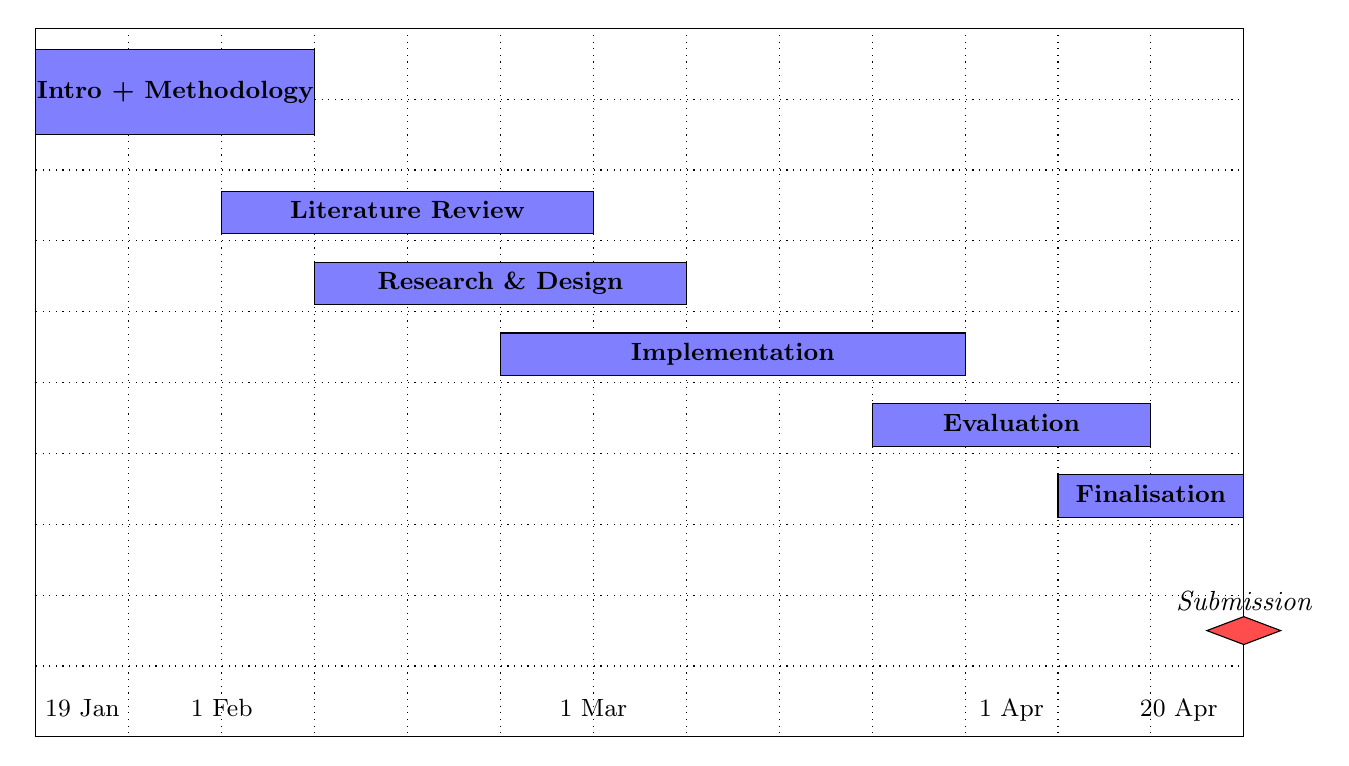
\begin{tikzpicture}
\begin{ganttchart}[
    hgrid,
    vgrid,
    x unit=1.18cm,
    y unit chart=0.9cm,
    bar height=0.6,
    bar label font=\small\bfseries,
    bar/.append style={fill=blue!50},
    milestone/.append style={fill=red!70},
    inline,
    bar label node/.append style={left=0.15cm, text=white},
    milestone label node/.append style={right=0.2cm, font=\small},
    y unit title=0pt,
    title height=0
]{1}{13}

\ganttbar[bar height=1.2]{Intro + Methodology}{1}{3} \\
\ganttbar[bar/.append style={fill=none, draw=none}]{}{1}{1} \\
\ganttbar{Literature Review}{3}{6} \\
\ganttbar{Research \& Design}{4}{7} \\
\ganttbar{Implementation}{6}{10} \\
\ganttbar{Evaluation}{10}{12} \\
\ganttbar{Finalisation}{12}{13} \\
\ganttbar[bar/.append style={fill=none, draw=none}]{}{1}{1} \\
\ganttmilestone{Submission}{13} \\
\ganttbar[bar/.append style={fill=none, draw=none}]{}{1}{1}

\end{ganttchart}

% Bottom axis labels at specific gridline positions
\node[below, font=\small] at (0.5*1.18, -8.4) {19 Jan};
\node[below, font=\small] at (2*1.18, -8.4) {1 Feb};
\node[below, font=\small] at (6*1.18, -8.4) {1 Mar};
\node[below, font=\small] at (10.5*1.18, -8.4) {1 Apr};
\node[below, font=\small] at (12.3*1.18, -8.4) {20 Apr};

\end{tikzpicture}
\caption{Project Gantt Chart (19 January to 20 April 2026)}
\label{fig:gantt-chart}
\end{figure}

Table~\ref{tab:project-milestones} lists the milestones with their specific deliverables and target dates. Each milestone represents a checkpoint where I will assess progress and decide whether to continue as planned or adjust course. The dates are targets rather than commitments. If a milestone slips, I will evaluate whether to compress subsequent work, reduce scope, or accept schedule delay.

\begin{table}[H]
\centering
\begin{tabularx}{\textwidth}{|l|l|L|L|}
\hline
\textbf{Phase} & \textbf{Date} & \textbf{Milestone} & \textbf{Deliverables} \\
\hline
1 & 19 Jan & Project Initiation & Repository setup, development environment configured \\
\hline
2 & 31 Jan & Initial Chapters & Introduction, Scope, Methodology chapters complete \\
\hline
3 & 21 Feb & Literature Review & Literature review chapter complete \\
\hline
4 & 28 Feb & Design Complete & Architecture diagrams, API specifications, data models \\
\hline
5 & 14 Mar & Core Components & Template analyser and data retrieval functional \\
\hline
6 & 28 Mar & MVP Complete & End-to-end generation pipeline operational \\
\hline
7 & 4 Apr & Testing Complete & Unit and integration tests passing; evaluation data collected \\
\hline
8 & 11 Apr & Evaluation Complete & Results analysis and evaluation chapter written \\
\hline
9 & 18 Apr & Document Finalised & All chapters complete, proofread, formatted \\
\hline
10 & 20 Apr & Submission & Final report submitted via QMPlus \\
\hline
\end{tabularx}
\caption{Project Milestones and Deliverables}
\label{tab:project-milestones}
\end{table}

\subsection{Risk Assessment and Mitigation}
\label{sec:risk-assessment}

Every project faces risks. The question is whether to identify them upfront and plan responses, or to discover them later when options are limited. I prefer the former.

I have categorised risks by source: technical risks (API limitations, LLM behaviour, template complexity), process risks (scope creep, time pressure), and external risks (API changes, compliance requirements). The mitigations focus on practical actions I can take rather than hoping problems do not occur.

Table~\ref{tab:risk-assessment} shows the risk register with likelihood and impact rated on a three-point scale (Low, Medium, High).

\begin{table}[H]
\centering
\begin{tabularx}{\textwidth}{|l|L|l|l|L|}
\hline
\textbf{ID} & \textbf{Risk Description} & \textbf{Likelihood} & \textbf{Impact} & \textbf{Mitigation Strategy} \\
\hline
R1 & API rate limits restrict data retrieval during development & Medium & Medium & Implement caching; use mock data for testing; stagger API calls \\
\hline
R2 & LLM outputs inconsistent or hallucinated content & High & High & Structured output schemas; validation layers; HITL review \\
\hline
R3 & Template analysis fails on complex slide layouts & Medium & High & Scope to common layouts; graceful degradation for unsupported elements \\
\hline
R4 & External API deprecation or changes & Low & High & Abstract API interactions; monitor changelogs; maintain fallback sources \\
\hline
R5 & Scope creep extends beyond POC boundaries & Medium & Medium & Strict MoSCoW prioritisation; regular scope reviews against requirements \\
\hline
R6 & Technical complexity exceeds available time & Medium & High & Iterative delivery; prioritise core pipeline; defer stretch goals \\
\hline
R7 & Data accuracy issues undermine credibility & Medium & High & Verification against manual retrieval; source attribution in outputs \\
\hline
R8 & Generated outputs violate compliance requirements & Low & High & Human review mandatory; disclaimer on all outputs; no PII processing \\
\hline
\end{tabularx}
\caption{Risk Assessment and Mitigation Strategies}
\label{tab:risk-assessment}
\end{table}

For high-impact risks, I have simple contingency rules. If LLM validation failures become frequent, I will reduce scope. If template extraction struggles with complex layouts, I will narrow the supported template types. If milestones slip by more than a week, I will drop the "Could have" requirements first.

\subsection{Ethics, Data Governance and Compliance}
\label{sec:ethics}

AI systems in financial services raise particular ethical concerns. The documents they help produce can influence major business decisions. Errors or bias in generated content could mislead clients or expose firms to liability. The design must address these concerns directly.

The system keeps humans in control of analytical judgements. Generated content is marked as AI-assisted, and HITL design ensures professional review before distribution. The system prioritises accuracy over completeness, flagging uncertainty rather than presenting unverified information as fact. When the system cannot retrieve data or has low confidence in generated content, it says so explicitly rather than filling gaps with plausible-sounding fabrications.

For data governance, the system processes only data needed for PB generation, with no retention of user inputs after sessions. All external data includes source attribution. The POC does not process personally identifiable information. Company data comes exclusively from public sources. This approach sidesteps many privacy concerns while still demonstrating the core functionality.

Regarding compliance, the HITL architecture meets EU AI Act requirements for human oversight \parencite{bis2024regulating}. Professional responsibility for final content remains with the banker. The system logs generation parameters and data sources to support audit requirements. If questions arise about how a particular output was generated, the logs provide a complete trail from input to output.

\subsection{Project Tracking}
\label{sec:tracking}

Progress will be tracked using GitHub Issues with a Kanban board (Backlog, In Progress, In Review, Done). Each functional requirement maps to one or more issues, providing traceability from requirements to implementation. Changes to scope or architecture will be documented in the issue history.

This approach serves two purposes. First, it keeps me organised during development. I can see at a glance what is done, what is in progress, and what remains. Second, it creates an audit trail for the dissertation. Anyone reviewing the work can trace how implementation decisions connected to requirements and how the project evolved over time.

\subsection{Reusability}
\label{sec:reusability}

Academic projects should produce reusable artefacts where possible. Code that only works for one specific case has limited value. I have designed the architecture with reusability in mind.

The architecture separates concerns into independent modules (template analysis, data retrieval, content planning, slide assembly), each with clean interfaces for standalone reuse. Someone interested only in template analysis could use that module without the rest of the system. Someone building a different kind of document generator could reuse the data retrieval layer.

All code will include Google-style docstrings, with a detailed README and architecture documentation. The codebase will be released under MIT License to minimise barriers to reuse. Configuration will be externalised so that adapting the system to different use cases does not require modifying source code.

\section{Preliminary Research and Design Documentation}
\label{sec:research-design}

{\small
\begin{longtable}{|p{3.8cm}|p{1.5cm}|p{6.8cm}|p{0.8cm}|}
\hline
\textbf{Source} & \textbf{Type} & \textbf{Summary} & \textbf{Link} \\
\hline
\endfirsthead
\hline
\textbf{Source} & \textbf{Type} & \textbf{Summary} & \textbf{Link} \\
\hline
\endhead
\hline
\endfoot
\hline
\endlastfoot

\rowcolor{headergray}\multicolumn{4}{|c|}{\textbf{Knowledge Management \& Knowledge Reuse}} \\
\hline
Markus (2001). Toward a Theory of Knowledge Reuse & Journal & Foundational theory on knowledge reuse; identifies four types of reuse situations and success factors & \href{https://doi.org/10.1080/07421222.2001.11045671}{\textcolor{blue}{\underline{Link}}} \\
\hline
Dalkir (2017). Knowledge Management in Theory and Practice & Textbook & Comprehensive KM textbook covering tacit/explicit knowledge and organisational memory systems & \href{https://mitpress.mit.edu/9780262036870/}{\textcolor{blue}{\underline{Link}}} \\
\hline

\rowcolor{headergray}\multicolumn{4}{|c|}{\textbf{Large Language Models}} \\
\hline
Zhao et al. (2023). A Survey of Large Language Models & Survey & Comprehensive survey on LLM development; covers GPT, LLaMA, PaLM families & \href{https://arxiv.org/abs/2303.18223}{\textcolor{blue}{\underline{Link}}} \\
\hline
Minaee et al. (2024). Large Language Models: A Survey & Survey & Reviews LLM characteristics, contributions, limitations, and augmentation techniques & \href{https://arxiv.org/abs/2402.06196}{\textcolor{blue}{\underline{Link}}} \\
\hline

\rowcolor{headergray}\multicolumn{4}{|c|}{\textbf{Retrieval-Augmented Generation}} \\
\hline
Lewis et al. (2020). RAG for Knowledge-Intensive NLP Tasks & Conference & Seminal RAG paper; combines parametric and non-parametric memory for factual generation & \href{https://arxiv.org/abs/2005.11401}{\textcolor{blue}{\underline{Link}}} \\
\hline
Gao et al. (2023). RAG for LLMs: A Survey & Survey & Comprehensive RAG survey covering taxonomy, methods, and applications & \href{https://arxiv.org/abs/2312.10997}{\textcolor{blue}{\underline{Link}}} \\
\hline
Chen et al. (2025). RAG and LLMs for Enterprise KM & Journal & Systematic review of 63 studies; 63.6\% use GPT models, 80.5\% use FAISS/Elasticsearch & \href{https://www.mdpi.com/2076-3417/16/1/368}{\textcolor{blue}{\underline{Link}}} \\
\hline
Fan et al. (2024). A Survey on RAG Meeting LLMs & Conference & KDD survey on integrating RAG with LLMs & \href{https://doi.org/10.1145/3637528.3671470}{\textcolor{blue}{\underline{Link}}} \\
\hline

\rowcolor{headergray}\multicolumn{4}{|c|}{\textbf{Agentic AI \& Autonomous Agents}} \\
\hline
Wang et al. (2024). A Survey on LLM-based Autonomous Agents & Journal & Foundational survey on LLM autonomous agents; proposes unified framework & \href{https://arxiv.org/abs/2308.11432}{\textcolor{blue}{\underline{Link}}} \\
\hline
Guo et al. (2024). LLM Based Multi-agents: A Survey & Conference & IJCAI survey on multi-agent LLM systems for complex problem-solving & \href{https://arxiv.org/abs/2402.01680}{\textcolor{blue}{\underline{Link}}} \\
\hline
Li et al. (2024). A survey on LLM-based multi-agent systems & Journal & Systematic review with five-component architecture framework & \href{https://arxiv.org/abs/2412.13093}{\textcolor{blue}{\underline{Link}}} \\
\hline

\rowcolor{headergray}\multicolumn{4}{|c|}{\textbf{LLM Tool Use \& Function Calling}} \\
\hline
Li (2025). A review of paradigms for LLM-based agents & Conference & Reviews tool use, planning, RAG, and feedback mechanisms & \href{https://arxiv.org/abs/2406.05804}{\textcolor{blue}{\underline{Link}}} \\
\hline

\rowcolor{headergray}\multicolumn{4}{|c|}{\textbf{Automated Document Generation}} \\
\hline
Zheng et al. (2025). PPTAgent: Generating Presentations & Conference & Two-stage edit-based presentation generation; introduces PPTEval framework & \href{https://arxiv.org/abs/2501.03936}{\textcolor{blue}{\underline{Link}}} \\
\hline
Liu et al. (2024). We Need Structured Output & Conference & Studies user needs for structured LLM outputs in professional contexts & \href{https://doi.org/10.1145/3613905.3650756}{\textcolor{blue}{\underline{Link}}} \\
\hline

\rowcolor{headergray}\multicolumn{4}{|c|}{\textbf{LLM Structured Output \& Prompt Engineering}} \\
\hline
Wu et al. (2024). LLM-Driven Structured Output: A Benchmark & Journal & Benchmark for structured outputs; compares fine-tuning, prompting, and RAG & \href{https://arxiv.org/abs/2411.00235}{\textcolor{blue}{\underline{Link}}} \\
\hline
Xu et al. (2025). Structured Data Generation with GPT-4o & Journal & Compares JSON, YAML, CSV prompt styles; JSON best for complex data & \href{https://arxiv.org/abs/2501.06466}{\textcolor{blue}{\underline{Link}}} \\
\hline

\rowcolor{headergray}\multicolumn{4}{|c|}{\textbf{LLM Hallucination \& Factual Accuracy}} \\
\hline
Huang et al. (2024). A Survey on Hallucination in LLMs & Journal & Comprehensive taxonomy of hallucination causes, detection, and benchmarks & \href{https://doi.org/10.1145/3703155}{\textcolor{blue}{\underline{Link}}} \\
\hline
Alansari \& Luqman (2025). LLM Hallucination Survey & Survey & Review of hallucination causes, detection, and mitigation strategies & \href{https://doi.org/10.1145/3703633}{\textcolor{blue}{\underline{Link}}} \\
\hline

\rowcolor{headergray}\multicolumn{4}{|c|}{\textbf{Human-in-the-Loop AI}} \\
\hline
Wu et al. (2022). A Survey of HITL for ML & Journal & Classifies HITL approaches: data processing, interventional training, system design & \href{https://doi.org/10.1016/j.future.2022.05.014}{\textcolor{blue}{\underline{Link}}} \\
\hline
Mosqueira-Rey et al. (2024). HITL ML: Role of the user & Journal & Discusses timing, frequency, and workload factors in interactive ML & \href{https://doi.org/10.1016/j.iot.2023.101048}{\textcolor{blue}{\underline{Link}}} \\
\hline
Rezaeighaleh et al. (2023). Ethical AI Based on HITL & Journal & Examines HITL for ethical AI development & \href{https://doi.org/10.1016/j.clsr.2023.105825}{\textcolor{blue}{\underline{Link}}} \\
\hline

\rowcolor{headergray}\multicolumn{4}{|c|}{\textbf{AI in Financial Services}} \\
\hline
Alghofaili et al. (2024). AI and ML in Banking Systems & Journal & Examines board role in AI adoption; Saudi Arabian banking sector & \href{https://doi.org/10.1016/j.heliyon.2024.e36884}{\textcolor{blue}{\underline{Link}}} \\
\hline
Kumari \& Tanwar (2023). AI/ML in Financial Services & Journal & Bibliometric analysis of 1,045 BFSI sector articles & \href{https://doi.org/10.1016/j.joitmc.2023.100137}{\textcolor{blue}{\underline{Link}}} \\
\hline
\rowcolor{headergray}\multicolumn{4}{|c|}{\textbf{AI Regulation \& Compliance}} \\
\hline
Zetzsche et al. (2024). Regulating AI in investment management & Journal & Discusses EU AI Act, GDPR, MiFID II implications for AI & \href{https://doi.org/10.1093/jfr/fjad012}{\textcolor{blue}{\underline{Link}}} \\
\hline

\rowcolor{headergray}\multicolumn{4}{|c|}{\textbf{Knowledge Worker Productivity}} \\
\hline
Brynjolfsson et al. (2023). Generative AI at Work & Working Paper & 14\% productivity increase from AI; greatest impact on novice workers & \href{https://doi.org/10.3386/w31161}{\textcolor{blue}{\underline{Link}}} \\
\hline
Noy \& Zhang (2023). Productivity effects of generative AI & Journal & Experimental study showing productivity improvements from ChatGPT use & \href{https://doi.org/10.1126/science.adh2586}{\textcolor{blue}{\underline{Link}}} \\
\hline
McKinsey (2012). The Social Economy & Report & Knowledge workers spend 20\% of time searching for information & \href{https://www.mckinsey.com/industries/technology-media-and-telecommunications/our-insights/the-social-economy}{\textcolor{blue}{\underline{Link}}} \\
\hline

\rowcolor{headergray}\multicolumn{4}{|c|}{\textbf{Vision-Language Models for Documents}} \\
\hline
Faysse et al. (2024). ColPali: Document Retrieval with VLMs & Research & Uses VLM for direct PDF image retrieval; introduces ViDoRe benchmark & \href{https://arxiv.org/abs/2407.01449}{\textcolor{blue}{\underline{Link}}} \\
\hline
Liao et al. (2024). DocVLM: Efficient Reader & Conference & Integrates OCR into VLMs; improves DocVQA from 56\% to 86.6\% & \href{https://arxiv.org/abs/2412.10493}{\textcolor{blue}{\underline{Link}}} \\
\hline

\rowcolor{headergray}\multicolumn{4}{|c|}{\textbf{Software Engineering Methodology}} \\
\hline
Anifa et al. (2024). Systematic Review on Agile Approach & Journal & Systematic review of agile methodology across industries & \href{https://doi.org/10.14569/IJACSA.2024.0150452}{\textcolor{blue}{\underline{Link}}} \\
\hline
Sommerville (2016). Software Engineering & Textbook & Standard software engineering reference; covers SDLC and methodologies & \href{https://www.pearson.com/en-us/subject-catalog/p/software-engineering/P200000003258}{\textcolor{blue}{\underline{Link}}} \\
\hline

\end{longtable}
}

\newpage
\section{Project Implementation and Outcomes}
\label{sec:implementation}

\newpage
\section{Evaluation and Conclusions}
\label{sec:evaluation-conclusions}

% --------------------------------------------
% BACK MATTER
% --------------------------------------------

% Bibliography
\newpage
\printbibliography[heading=bibintoc]

% Appendices
\newpage
\begin{appendices}

% TODO: Include risk assessment table

% TODO: Include Gantt chart or project timeline

% TODO: Map project to apprenticeship Knowledge, Skills, and Behaviours

\end{appendices}

\end{document}
